%\begin{refsection}
\section{Introduction}


Modern deep neural networks (DNNs) are complex,
and often contain millions of parameters spanning
dozens or even hundreds of layers~\cite{he2016deep,huang:2017}.
%
This complexity translates into substantial memory and runtime costs
on hardware platforms at all scales.
%
Recent work has demonstrated that DNNs are often over-provisioned and can be compressed without appreciable loss of accuracy.
Model compression can be used to
reduce both model memory footprint and inference latency using techniques such as
weight pruning~\cite{han2015learning,luo2017thinet},
quantization~\cite{gupta2015deep}, and low-rank
factorization~\cite{jaderberg2014speeding,denton2014exploiting}.
%
Unfortunately, the requirements of
different {\em compression contexts}---DNN structure,
target hardware platform, and the user's optimization objective---are often in conflict.
%
The recommended compression strategy for reducing inference latency
may be different from that required to reduce total memory footprint.
%
For example, in a Convolutional Neural Network (CNN),
reducing inference latency may require pruning filters to realize speedups on real hardware~\cite{li2016pruning}, while reducing memory footprint may be accomplished by zeroing out individual weights.
%
Similarly, even for the {\em same optimization objective},
say reducing inference latency, one may employ filter pruning for a CNN,
while pruning 2-D blocks of non-zero weights~\cite{gray:2017} for a
language modeling network such as Transformer~\cite{vaswani:2017},
since the latter has no convolutional layers.
%
Thus, it is crucial to enable convenient expression of 
alternative compression schemes, yet
none of today's model compression approaches help the designer
tailor compression schemes to their needs.


\begin{figure}[!h]
\centering
%\fbox{\rule{0pt}{2in} \rule{0.9\linewidth}{0pt}}
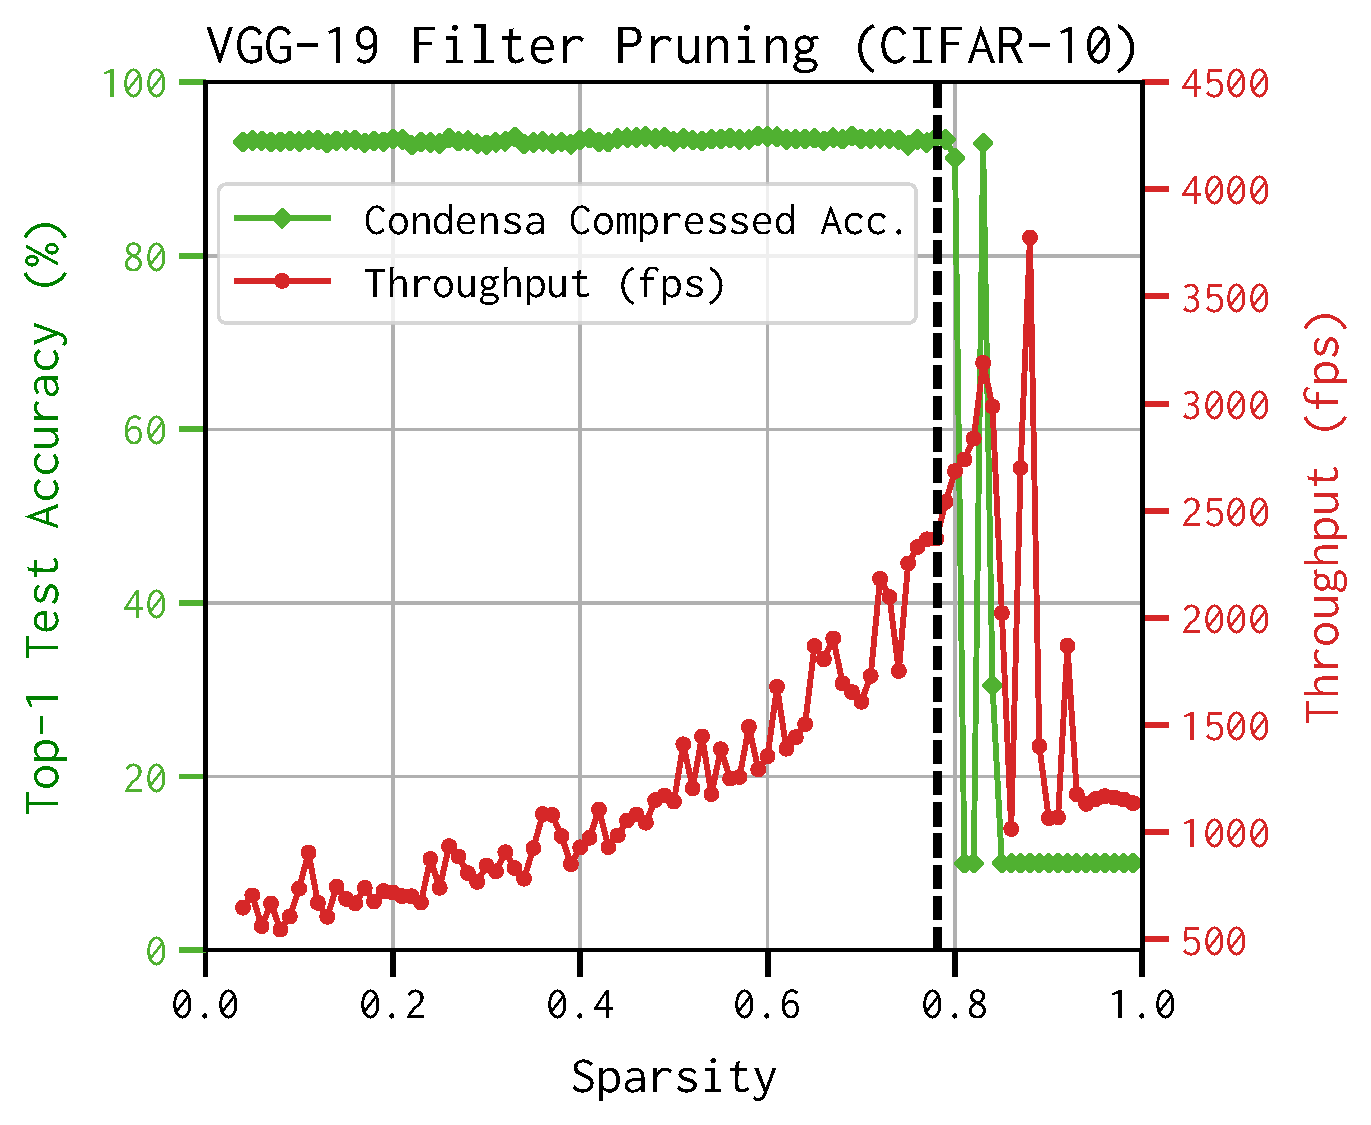
\includegraphics[width=0.5\linewidth]{img/vgg19_bn_filter_intro_v2.pdf}
%\vspace{-10pt}
\caption{Top-1 test accuracy (green) and throughput (red) vs.\ sparsity for VGG-19 on CIFAR-10.
\algoName is designed to solve constrained optimization problems of the form ``maximize throughput, with a lower bound on accuracy". In this case, \algoName automatically discovers a sparsity (vertical dashed line) and compresses the model to this sparsity,
improving throughput by $2.59\times$ and accuracy by $0.36\%$.
}
\vspace{-10pt}
\label{fig:vgg-intro}
\end{figure}

%Current approaches to model compression
%also require manual specification of compression hyperparameters, such
%as the target sparsity ratio, which is the proportion of zero-valued parameters in %the
%compressed model vs.\ the original.
%
Current approaches to model compression
also require manual specification of compression hyperparameters, such
as {\bf target sparsity}---{\em the proportion of zero-valued parameters in the
compressed model vs.\ the original.}
%
However, with current approaches, finding the best sparsity 
often becomes a trial-and-error search, with
each such trial having a huge cost (often multiple days for large models such as BERT) and involving training the compressed model to convergence,
only to find (in most cases) that the compression objectives are not met.
%
The main difficulty faced by such unguided approaches is
that sparsities 
vary unpredictably with changes in the compression context,
making it very difficult to provide users with any guidelines, whatsoever.
%
Therefore, automatic and {\em sample-efficient} approaches that minimize the number of trials are crucial
to support the needs of designers who must adapt
a variety of neural networks to a broad spectrum of platforms targeting a wide
range of tasks.

To address the above-mentioned problems of flexible expression of compression strategies, automated compression hyperparameter inference, and sample efficiency, we introduce \algoName, a new framework for programmable model compression. As an illustration of the level of automation provided by \algoName,
consider the problem of improving the
inference throughput of VGG-19~\cite{simonyan2014very} on the CIFAR-10 image
classification task~\cite{krizhevsky2014cifar}.
%
Since VGG-19 is a convolutional neural network, one way to improve its
inference performance on modern hardware such as GPUs is by pruning
away individual convolutional filters~\cite{he2018progressive}.
%
Figure~\ref{fig:vgg-intro} shows the accuracy and throughput obtained
by \algoName on this task.
%
Here, we plot the compressed model's top-1 test accuracy and throughput as a function of the sparsity (green and red lines,
respectively).\footnote{Note that these curves are not known a priori and
are often extremely expensive to sample;
they are only plotted here to better place the obtained solution in context.}
%
\algoName's solution corresponds to a sparsity of $0.79$
and is depicted as the vertical dashed line.
%
This result is significant for two reasons: (1) using the \algoName library,
the filter pruning strategy employed for this experiment was expressed in
less than 10 lines of Python code, and (2) the optimal sparsity of
$0.79$ that
achieves throughput and top-1 accuracy improvements of $2.59\times$ and $0.36\%$, respectively,
was obtained automatically by \algoName using a sample-efficient constrained
Bayesian optimization algorithm.
%
Here, the user didn't have to specify any
sparsities manually, and instead only had to define a domain-specific
objective function to maximize (inference throughput, in this case).

\begin{figure*}[!t]
\centering
  % \includegraphics[width=0.8\textwidth,height=10cm]{CVPR2021/img/FinalIntroFigure.pdf}
  \includegraphics[width=\textwidth]{img/FinalIntroFigure.pdf}
  \caption{Overview of our CIE reduction framework using label preservation-aware loss functions.}
  \label{fig:overview}
\end{figure*}

%\end{refsection}